% !TeX spellcheck = de_DE

\documentclass[skip,a4paper]{article}

\usepackage{ucs}
\usepackage[utf8x]{inputenc}
\usepackage[T1]{fontenc}
\usepackage{amsmath}
\usepackage{amsfonts}
\usepackage{amssymb}
\usepackage[top=1cm,bottom=1cm,right=2cm,left=1cm]{geometry}
\usepackage{titlesec}
\usepackage{array}
\usepackage{enumitem}
%% URLs
\usepackage{hyperref}
\usepackage{url}
\usepackage{ulem} % em is underlined

%% Graphics and colors
\usepackage{tikz} % Round corner on picture
\usepackage{color} % enable color
\usepackage{xcolor} % Define own colors
\usepackage{graphicx} % Include picts.

%% Fonts
% cf http://www.tug.dk/FontCatalogue/seriffonts.html
\usepackage[default,osfigures,scale=0.95]{opensans}
% Symbols
\usepackage{marvosym}


%-----Liens PDF-----%
\hypersetup{
	%backref=true, %permet d'ajouter des liens dans...
	%pagebackref=true,%...les bibliographies
	%hyperindex=true, %ajoute des liens dans les index.
	colorlinks=true, %colorise les liens
	breaklinks=true, %permet le retour à la ligne dans les liens trop longs
	urlcolor=black, %couleur des hyperliens
	linkcolor=black, %couleur des liens internes
	%bookmarks=true, %créé des signets pour Acrobat
	%bookmarksopen=true, %si les signets Acrobat sont créés,
	%les afficher complètement.
	pdftitle={\title}, %informations apparaissant dans
	pdfauthor={\author}, %dans les informations du document
	pdfsubject={\subject} %sous Acrobat.
}

\makeatletter

\pagestyle{empty}

\def\UrlFont{\em} % url are `em`, and `em` is underlined with ulem

\titleformat{\section}{\LARGE\bfseries\color{redcv}}{\thesection}{1em}{}[{\titlerule[0.8pt]}]
\titleformat{\subsection}{\normalfont\Large\bfseries}{\thesubsection}{1em}{}

\titlespacing*{\section}{0pt}{2ex plus 0.4ex minus .2ex}{1.3ex plus .2ex}
\titlespacing*{\subsection}{50pt}{2ex plus 0.4ex minus -0.2ex}{0.5ex plus .2ex}

\newcommand{\itemcv}[2]{\textbf{\color{graycv}#1} & #2 \tabularnewline}
	
\newcolumntype{P}[1]{>{\raggedright}p{#1}}
\makeatother	
\usepackage[german]{babel}
\def\subject{Olivier CHURLAUD - Lebenslauf}
\def\title{Olivier CHURLAUD - Lebenslauf}
\def\author{Olivier CHURLAUD}
\def\place{Berlin}

\makeatletter
	\definecolor{redcv}{HTML}{C5000B}
	\definecolor{graycv}{HTML}{666666}
	\def\scale{0.94}
	\def\descripscale{0.8}
	\def\datescale{0.13}
	\renewcommand{\arraystretch}{1.7}
\makeatother

\begin{document}
\fontsize{8.5}{9.5}
\selectfont

\begin{minipage}[c]{\linewidth}
	\begin{minipage}[c][4cm]{2.6cm}
		~\\~\\
		\begin{tikzpicture}
			\begin{scope}
				\clip [rounded corners=.5cm] (0,0) rectangle coordinate (centerpoint) (2.4,3cm); 
				\node [inner sep=0pt] at (centerpoint) {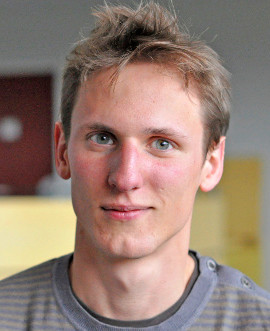
\includegraphics[width=2.4cm]{img/ID_ochurlaud}}; 
			\end{scope}
		\end{tikzpicture}
		\vfill
		~
	\end{minipage}
	\begin{minipage}[c][4cm]{5.5cm}
		\textbf{Olivier CHURLAUD}

		\begin{itemize}[itemsep=0.5ex,leftmargin=3ex]
			\footnotesize
			\item[\bfseries @] \url{olivier@churlaud.com}
			\item[\bfseries \color{blue} in] {\scriptsize\url{ fr.linkedin.com/in/olivierchurlaud/}}
			\item[\Telefon]+49 (0)157 52931348
			\item[\Letter] Weitlingstr. 101 \\
			10 317 BERLIN \\ 
			DEUTSCHLAND
			10 317 BERLIN
			\item[$\bullet$] Geburtsdatum: 07.04.1992
			\itemsep -2pt
			\item[$\bullet$] Familienstand: Ledig
			\item[$\bullet$] Atheist
		\end{itemize}
	\end{minipage}
	\begin{minipage}[c][4cm]{10cm}
		\begin{minipage}[c]{7.10cm}
			
\includegraphics[width=6.5cm]{img/ecl}
		\end{minipage}
		\hfill
		\begin{minipage}[c]{2.5cm}
			
\includegraphics[width=2.1cm]{img/tuberlin}
		\end{minipage}
		
		\vfill
		
		\centering
		{
			\setlength{\parskip}{10pt plus 1pt minus 1pt}
			{\LARGE Studentischer Mitarbeiter}
			
			{\large Masterstudent im Bereich \textit{Digitale Nachrichtübertragung} und \textit{Signalverarbeitung}}
		}
	\end{minipage}
\end{minipage}

\vfill
\begin{minipage}{\linewidth}
	~
	\hfill
	\begin{minipage}{\scale\linewidth}
	~
		\section*{Schulausbildung und Studium}
		\begin{tabular}{p{\datescale\linewidth} P{\descripscale\linewidth}}
			\itemcv{2014 -- 2016}{
					\textbf{Doppel Diplom an der TU Berlin: M.Sc. Elektrotechnik}\\
					Studienschwerpunkte: Kommunikationssysteme, Codierungstheorie, Nachrichtübertragung
				}
			\itemcv{2012 -- 2016}{
					 \textbf{Hauptstudium an der \'Ecole Centrale de Lyon: Ingenieur Grande \'Ecole für Generalisten}\\
					 Studienschwerpunkte: Informatik und Elektronik
				}
			\itemcv{2010 -- 2012}{
					 \textbf{Vorbereitungsklasse für die Aufnahme an eine Grande \'Ecole}: Selektive Aufnahmeprüfung
				}
		\end{tabular}
		
		\section*{Erfahrungen}
		\subsection*{Projektführung}
		
		\begin{tabular}{p{\datescale\linewidth} P{\descripscale\linewidth}}
			\itemcv{2013 -- 2014}{
					\textbf{Forschungsprojekt: Entwicklung eines Kommunikationsmoduls WPAN-WLAN} \\
					Zusammenarbeit mit dem Labor INL (Lyon) \\
					\textit{C Programmierung -- KICAD -- Microchip Mikrocontrollers}
				}
			\itemcv{2012 -- 2013}{
				\textbf{Vorsitzender des gemeinnütziger Vereins ECLAIR} \\
				Verein, der die Informatik und das Netzwerk des Campus verwaltet
			}
			\itemcv{~}{
				\textbf{Schulprojekt : Erstellung eines Messgerätes um Niederfrequenzfelder zu messen} \\
				Zusammenarbeit mit dem Labor Ampère (Lyon) \\
				\textit{MATLAB Programmierung / Anwendung eines Magnetometer}
			}
			\itemcv{2009-2010}{
				\textbf{Forschungsproject in Teilchenphysik mit CERN und IN2P3}
				2 mal den ersten Preis in der wissenschaftlichen Aufnahmeprüfung gewonnen
				\textit{Experimente / Populärwissenschaftliche Darstellungen}
			}
			
			\itemcv{2008 -- 2009}{
				\textbf{Projet d'Atelier d'écriture en partenariat avec l'OuLiPo} (Ouvroir de Littérature Potentielle : groupement	d'écrivains qui travaille en se choisissant des contraintes de fond et de forme)
			}
		\end{tabular}
				
		\subsection*{Berufspraktische Erfahrungen}
		
		\begin{tabular}{p{\datescale\linewidth} P{\descripscale\linewidth}}
			\itemcv{Mai-Aug. 2014}{
				\textbf{Forschungpraktikum mit Francesco P. Andriulli (Telecom Bretagne)}\\
				Analyse und Entwicklung von Techniken für Experimente und Computation für EEG.
			}
		\end{tabular}

		\section*{Besondere Fähigkeiten}

		\begin{tabular}{p{\datescale\linewidth} P{\descripscale\linewidth}}
			\itemcv{Management}{Projekt Führer, Team Koordination}
			\itemcv{Elektrotechnik}{Informationstheorie, Codierungstheorie (Quellen- und Kanalcodierung), Signalverarbeitung}
			\itemcv{Informatik}{
				Programmierung, Machine Learning -- \textbf{Nerzwerkverwaltung} Linux, Bridging, VLAN, Virtualisierung KVM, Apache2 -- \textbf{Programmierung} MATLAB, C/C++, MySQL, Python, \LaTeX
			}
			\itemcv{Sprache}{
				\textbf{Französisch} (Muttersprache), \textbf{Englisch} (sehr gut Kenntnisse: 12 Jahre), \textbf{Deutsch} (Niveau B2 das
				europäischen Referenznahmens: 12 Jahre, Seit 8 Monate in Berlin)
			}
			\itemcv{Andere}{Führerschein Klasse B}
		\end{tabular}
		
		\section*{Freizeitbeschäftigen}
				
		\begin{tabular}{p{\datescale\linewidth} P{\descripscale\linewidth}}
			\itemcv{Kultur}{Literatur (Klassische Literatur und Nouveau Roman)}
			\itemcv{}{Musik, Kino (Autorenfilme und Filme aus dem Vierziger und Fünfziger Jahren)}
			\itemcv{Sport}{Gebirgssports (Ski, Klettern, Wanderung)}
	\end{tabular}
	\end{minipage}
\end{minipage}
\vfill
\begin{minipage}[t][50pt]{150pt}
	 \vspace{0pt}
	 \place, den \today,
\end{minipage}
\begin{minipage}[t]{200pt}
	 \vspace{0pt}\includegraphics[width=100pt]{img/signature.png}
\end{minipage}
\end{document}